\documentclass[09pt,letterpaper]{article}
\usepackage[lmargin=2.2in,rmargin=0.7in,tmargin=1.0in,bmargin=1.0in]{geometry}
\usepackage{notes}
\begin{document}

\begin{center}
\Large\textbf{1.7 - Population Models}\\
\normalsize (Section 1.5.1)
\end{center}

%-------------------------------------------------------------
\section{Basic Growth Model}

Thomas Malthus was an essayist in the late 1700s who proposed a simple
mathematical model for population growth. The model is
$P'=rP,$
where $P(t)$ is the population at time $t$ and $r$ is a constant.



\subsection{Model Assumption}

Let $P(t)$ denote the population of a species at time $t$. The time variable
$t$ may be measured in minutes, days, years, etc. Suppose the population grows at a fixed percentage rate $r$ per unit time.
Over a small time interval $\Delta t$, we approximate the change in
population by
\[
\underbrace{P(t+\Delta t) }_{\small\begin{array}{c}
    \text{future}\\
    \text{pop.}
  \end{array}} 
\;\,\approx 
\underbrace{P(t)}_{\small\begin{array}{c}
    \text{current}\\
    \text{pop.}
  \end{array}}
  +\;\;
\underbrace{r\; \Delta t P(t)}_{ \small \begin{array}{c}
    \text{growth}\\
    \text{factor}
  \end{array}}
\]
With a little rearrangement, we can write this as
\[
\frac{P(t+\Delta t)-P(t)}{\Delta t}
\approx rP(t).
\]
In the limit as $\Delta t\to0$, we obtain the continuous \textbf{basic growth model}
\[
\frac{dP}{dt}=rP.
\]
The idea behind the model is simple: if the population is large, there are
more individuals capable of reproducing. Therefore, the population growth
rate increases with population size.

\subsection{Parameter $r$}
The parameter $r$ is called the \textbf{intrinsic growth rate}. It represents
the net per-capita growth rate of the population and may be interpreted as $r = \text{birth rate} - \text{death rate}$. External factors like migration should not be aggregated into $r$. The units of $r$ are inverse time. For example,
\[
r=0.15\;\text{month}^{-1}
\]
corresponds to a growth rate of $15\%$ per month.
We should now be able to translate descriptions of population growth into
differential equation models.

\begin{example}[1]{
For each species, write the basic growth model that describes its population.
\begin{itemize}
    \item A population of rabbits grows at a rate of $30\%$ per
    month.

    \item A population of bacteria roughly triples per
    minute.
\end{itemize}
}

\begin{itemize}

\item Let $R(t)$ be the rabbit population after $t$ months. Since the intrinsic
growth rate is $30\%$ per month, $r=30\%=0.3$.
Therefore, the model is
\[
\boxed{
R'=0.3R.
}
\]

\item Let $B(t)$ be the bacteria population after $t$ minutes. Population tripling means the same as a $200\%$ growth rate. Therefore, the intrinsic growth rate is $r=200\%=2$. The model is
\[
\boxed{
B'=2B.
}
\]
\end{itemize}
\end{example}


\subsection{An Issue with the Model}

Suppose we model a growing population by
\[
P'=rP, \qquad P(0)=P_0,
\]
where $r>0$. The solution is
$$
P(t)=P_0e^{rt}.
$$
This can be a reasonable model over short time spans. However, 
\[
\lim_{t\to\infty}P(t)
=
\lim_{t\to\infty}P_0e^{rt}
=
\infty.
\]
In other words, the model predicts that the population will grow
\textit{without bound}. The problem is that the basic growth model assumes the same growth rate regardless of population size. In reality, resources such as food, space,
and water are limited. As a population becomes large, these limitations
begin to slow its growth.

Thus, the basic growth model can be useful over short time spans, but it is
usually unrealistic over long time spans. We need a better model that
accounts for limited resources. We can create a more realistic model by modifying the basic one.

%-------------------------------------------------------------

\section{Logistic Growth Model}
In the 1830s, Belgian mathematician Verhulst developed a model to describe
self-limiting population growth, generalizing the earlier exponential growth
model of Malthus by incorporating a sustainable population level known as the
carrying capacity.

\subsection{Carrying Capacity}

Every population should have a soft upper bound due to the limited resources
in an ecosystem. Let $K>0$ represent a sustainable population level. The
parameter $K$ is called the \textbf{carrying capacity}, and it has the same
units as population. We want three things to be true:
\begin{itemize}
    \item If the population is below $K$, the population should rise.
    \item As the population approaches $K$, its growth should slow down.
    \item If the population is above $K$, the population should fall.
\end{itemize}

\subsection{The Model}
To enforce the three properties of the carrying capacity $K$, we modify the basic growth model as follows:
$$
P' =rP \quad \rightarrow \quad P' = rP\left(1-\frac{P}{K}\right).
$$
The effect of the new factor  $1-\tfrac{P}{K}$ depends on the population level with respect to $K.$ The effects are summarized in the table below. 
We call
\[
P'=rP\left(1-\frac{P}{K}\right)
\]
the \textbf{logistic growth model}. It is a more realistic extension of the
basic growth model because the growth rate now depends on the size of the
population relative to its carrying capacity. Since this is an autonomous equation, we can analyze the population behavior
without explicitly solving the DE.
\begin{figure}
    \centering
\[
\begin{array}{c|c|c|c}
\text{Population} & 1-\frac{P}{K} & \text{Sign of }P' & \text{Effect}\\
\hline
P\ll K & \approx 1 & + & \text{nearly basic growth }P'\approx rP \\[4pt]
0<P<K  & >0 &+& \text{population grows}\\[4pt]
P=K & 0 & 0 & \text{no population growth}\\[4pt]
P>K & <0 & - & \text{population declines}
\end{array}
\]
\caption{We consider four different population levels. As population $P(t)$ grows from very small to above $K$, the sign of $P'$ changes from positive to zero to negative.}
\end{figure}

\begin{example}[2]{    
A fish population follows logistic growth with an intrinsic growth rate $r=0.4$ per year and a carrying capacity of $K=10000$ fish.
Suppose the initial population of fish is $P(0)=2000$. What happens to the population in the long run? What if the initial population is $12000$?
}

\paragraph{Set up the model.} This is a logistic model with $r=0.4$ per year and $K=10000$ fish. The initial condition is $P(0)=2000$ fish. We may write the model as the following IVP: 
$$
\begin{dcases}
    P' = 0.4\,P\left(1-\tfrac{P}{10000}\right)\\
    P(0)=2000
\end{dcases}
$$
We can solve this equation, but we will instead use the graphical methods that we learned on Day 06.

\paragraph{Find the equilibria and their stability}
The equilibria can be found by setting the RHS equal to zero and solving for $P$:
\begin{align*}
     f(P)&=0.4\,P\left(1-\tfrac{P}{10000}\right)\\
        0&=0.4\,P\left(1-\tfrac{P}{10000}\right)\\
     \implies&P^*=0, \quad P^*= 10000
\end{align*}
The $P'$ versus $P$ graph and phase line are shown below. Since negative
populations are not physically meaningful, we only consider $P\geq0$.
\begin{figure}[H]
    \centering
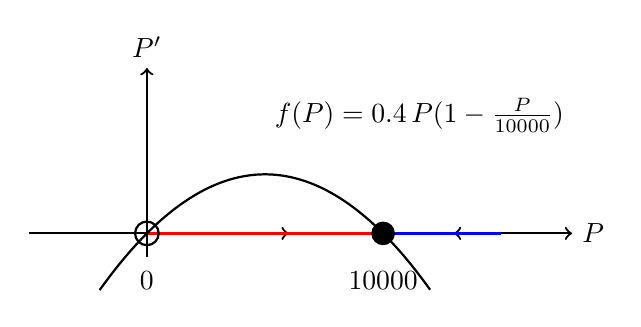
\begin{tikzpicture}[scale=3]
\begin{scope}
    % Axes
        % arrows: x<0 left
    % \draw[->,thick] (-0.3,0) -- (-0.4,0);
    % arrows: 0<x<1 right
    \draw[->,thick] (0.4,0) -- (.6,0);
    % arrows: x>1 left
    \draw[->,thick] (1.4,0) -- (1.3,0);
    % Axes
    \draw[->,thick] (-0.5,0) -- (1.8,0) node[right] {$P$};
    % \draw[very thick,blue] (-0.5,0) -- (0,0);
    \draw[very thick,blue] (1,0) -- (1.5,0);
    \draw[very thick,red] (0,0) -- (1,0);
    \draw[->,thick] (0,-.1) -- (0,0.7) node[above] {$P'$};
    % Curves x(t) = C e^{-t}
    \draw[thick,domain=-0.2:1.2,samples=100] plot (\x,{ \x*(1-\x)});
    \node[right] at (0.5,0.5) {$f(P)=0.4\,P(1-\frac{P}{10000})$};
        \node[below] at (0,-0.12) {$0$};
    \node[below] at (1,-0.12) {$10000$};
        \fill (1,0) circle (0.05);
        \draw[thick] (0,0) circle (0.05);\textbf{}
\end{scope}
\end{tikzpicture}
\end{figure}

The phase line shows that $P^*=0$ is unstable and $P^*=10000$ is stable.

\paragraph{Interpret the solutions.}
If $P(0)=2000$ fish, then $0<P_0<10000$, 
so $P'>0$ and the population increases toward $10000$. If $P(0)=12000$, then $P_0>10000$, so $P'<0$ and the population decreases toward $10000$. The solution curves are plotted below. 

\begin{figure}[H]
\centering
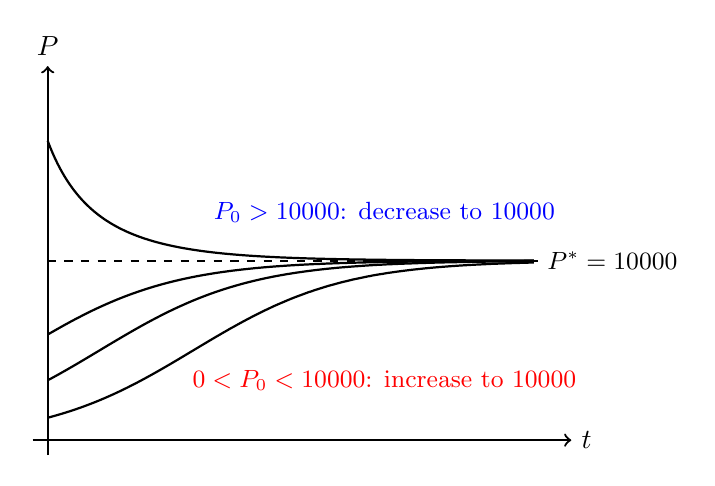
\begin{tikzpicture}[scale=0.95]
    % axes
    \draw[->,thick] (-0.2,0) -- (7,0) node[right] {$t$};
    \draw[->,thick] (0,-0.2) -- (0,5) node[above] {$P$};

    % equilibria: x=0 and x=1
    \draw[dashed,thick] (0,0) -- (6.6,0);
    % \node[left] at (0,0) {$0$};
    \draw[dashed,thick] (0,2.4) -- (6.6,2.4);
    % \node[left] at (0,2.4) {$1$};
    % (i) 0 < x0 < 1 : increasing to 1
    \draw[thick,domain=0:6.5,samples=200]
        plot (\x,{2.4*(1/(1 + 7*exp(-\x)))});
    \draw[thick,domain=0:6.5,samples=200]
        plot (\x,{2.4*(1/(1 + 2*exp(-\x)))});
    \draw[thick,domain=0:6.5,samples=200]
        plot (\x,{2.4*(1/(1 + 0.7*exp(-\x)))});

    % (ii) x0 > 1 : decreasing to 1  (A<0)
    \draw[thick,domain=0:6.5,samples=200]
        plot (\x,{2.4*(1/(1 - 0.4*exp(-\x)))});
    % \draw[thick,domain=0:6.5,samples=200]
    %     plot (\x,{2.4*(1/(1 - 0.7*exp(-\x)))});
    % \draw[thick,domain=0:6.5,samples=200]
    %     plot (\x,{2.4*(1/(1 - 0.85*exp(-\x)))});

    % labels near the right side
    \node[right] at (6.55,2.4) {\small  $P^*=10000$};


    % optional zone notes (remove if you want it cleaner)
    \node[blue] at (4.5,3.05) {\small $P_0>10000$: decrease to $10000$};
    \node[red] at (4.5,0.8) {\small $0<P_0<10000$: increase to $10000$};
\end{tikzpicture}
\end{figure}
Thus, in either case,
\[
\boxed{\lim_{t\to\infty}P(t)=10000.}
\]
The fish population stabilizes at 10,000 fish regardless of the starting condition. The carrying capacity is therefore a sustainable population level, not a hard upper bound. 
\end{example}


%-------------------------------------------------------------

% \subsection{Explicit Solution}
% This IVP for logistic growth 
% \[
% P' = rP\left(1-\frac{P}{K}\right), \qquad P(0)=P_0,
% \]
% can be solved using separation of variables and partial fraction decomposition. The exact solution is of the form 
% \[
% \boxed{
% P(t)=\frac{K}{1+Ce^{-rt}}, \quad\text{where }  C = \frac{K-P_0}{P_0}.
% }
% \]
% The $P(t)$ is called the \textbf{logistic function}. It is frequently used to model population. When plotted, it resembles an slated $S$-shape. In the limit as $t\rightarrow\infty$ the exponential term decays and we have 
% $$
% \lim_{t\rightarrow\infty} P(t) = \lim_{t\rightarrow\infty } \frac{K}{1+Ce^{-rt}} = \frac{K}{1+0}=K.
% $$
% \begin{figure}[H]
% \centering
% \begin{tikzpicture}[scale=0.9]
%     % axes
%     \draw[->,thick] (-0.2,0) -- (7,0) node[right] {$t$};
%     \draw[->,thick] (0,-0.2) -- (0,3.2) node[above] {$P$};

%     % K line
%     \draw[dashed,thick] (0,2.6) -- (6.7,2.6);
%     \node[left] at (0,2.6) {$K$};

%     % curves: P=K/(1 + A e^{-rt}) scaled
%     % choose r=1 for picture, K=2.6
%     \draw[thick,domain=0:6.5,samples=200]
%         plot (\x,{2.6*(1/(1 + 6*exp(-\x)))});
%     \draw[thick,domain=0:6.5,samples=200]
%         plot (\x,{2.6*(1/(1 + 2*exp(-\x)))});
%     \draw[thick,domain=0:6.5,samples=200]
%         plot (\x,{2.6*(1/(1 + 0.6*exp(-\x)))});

%     \node[right] at (5.0,2.15) {\small solutions approach $K$};
% \end{tikzpicture}
% \caption{These are the plots of the logistic function for a few different values of $0<P_0<K$. The key features to note are its $S$-shaped bend and its limiting value.}
% \end{figure}


%-------------------------------------------------------------
\section{Harvesting}

%-------------------------------------------------------------
\subsection{Basic Growth with Harvesting}

Recall that the basic growth model is
\[
P'=rP,
\]
where $r$ is the intrinsic growth rate. The term $rP$ represents
\textit{percentage-based growth}: as the population increases, the number of
individuals added per unit time also increases.

Now suppose that individuals are harvested from the population at a \textit{constant
rate} $h>0$. Unlike $rP$, the harvesting rate does not depend on the size of
the population. It is a \textit{flat rate}. For example, harvesting
$h=100$ fish per month means that 100 fish are removed each month, regardless
of the current fish population. Combining intrinsic growth with constant harvesting gives
\[
P'=rP-h.
\]
The parameter is called the \textbf{harvesting rate}, and it has units of population per unit time. Let's practice setting up a model. 

\begin{example}[3]{
A deer population has an intrinsic growth rate of $12\%$ per year.
Hunters remove deer from the population at a rate of $5$ deer per month.
Write a differential equation model for the deer population, where $t$ is
measured in years.
}

Since $t$ is measured in years, both rates must be expressed in terms of
years. The intrinsic growth rate is
\[
r=0.12 \text{ per year}.
\]
The harvesting rate is
\[
h
=
5\,\frac{\text{deer}}{\text{month}}
\left(
\frac{12\,\text{months}}{1\,\text{year}}
\right)
=
60\,\frac{\text{deer}}{\text{year}}.
\]
Therefore, the model is
\[
\boxed{
P'=0.12P-60.
}
\]
\end{example}

%-------------------------------------------------------------
\subsection{Critical Population Threshold}

Consider the basic growth model with constant harvesting:
\[
P'=rP-h,
\qquad r,h>0.
\]
This autonomous equation has one equilibrium 
\begin{align*}
P^* &= \frac{h}{r}.
\end{align*}
To determine its stability, consider the function $f(P)=rP-h$. We can plot $f(P)$ on the $P'$ versus $P$ graph. This is an increasing linear function of $P$ that crosses the $P$-axis at $P=h/r$. We may draw the phase line directly on the $P$-axis.
\begin{figure}[H]
\centering
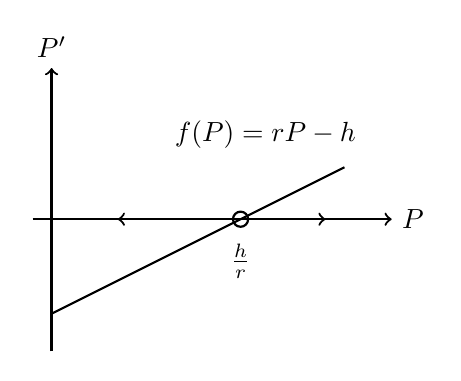
\begin{tikzpicture}[scale=2.4]
    % Phase arrows
    \draw[<-,thick] (0.35,0) -- (0.55,0);
    \draw[->,thick] (1.25,0) -- (1.45,0);
    % P-axis
    \draw[->,thick] (-0.1,0) -- (1.8,0) node[right] {$P$};
    % P'-axis
    \draw[->,thick] (0,-0.7) -- (0,0.8) node[above] {$P'$};
    % f(P)
    \draw[thick,domain=0:1.55,samples=100] plot (\x,{-0.5 + 0.5*\x});
    % Equilibrium
    \draw[thick] (1,0) circle (0.04);
    \node[below] at (1,-0.08) {$\frac{h}{r}$};
    % Function label
    \node[right] at (0.6,0.45) {$f(P)=rP-h$};

\end{tikzpicture}
\caption{$P'$ versus $P$ for the basic growth model with constant harvesting.}
\end{figure}
The arrows point away from $P^*=h/r$, so the equilibrium is unstable. Depending on whether the initial population $P_0=P(0)$ is below or above the equilibrium, the behavior of the population changes. 
\begin{itemize}
    \item If $0<P_0<\frac{h}{r}$, then $P'<0$ and the population decreases. 
    \item If $P_0>\frac{h}{r}$, then $P'>0$ and the population increases.
\end{itemize}
Thus, the equilibrium $P^*=\frac{h}{r}$ acts as a \textbf{critical population threshold}. Below this threshold, harvesting outpaces intrinsic population growth. Above this threshold, intrinsic population growth outpaces harvesting.

%-------------------------------------------------------------


% \subsection{Example}
% Suppose a fish farm has a population that grows intrinsically by $20\%$ per month. The farmers plan to harvest the fish at a rate 100 fish per week. Write a model for the fish population and describe the long-term effects of harvesting based on the initial population of fish.

% \paragraph{Write the model.}
% We let $P(t)$ = population of fish at $t$ months. The intrinsic growth rate is $r=0.2$ per month. The harvesting rate is given in $h=$100 fish per week. This has to converted to fish per months. Multiplying by four gives $h=400$ fish per month. Therefore, the model is 
% $$
% P' = 0.2\,P\,-400.
% $$
% \paragraph{Equilibria and Stability.} 
% The autonomous DE has only one equilibrium at $P^* = 400/0.2 =2000$. The RHS $f(P)=0.2 P-400$ is just a straight line. The $P'$ versus $P$ graph is plotted below. On the same plot, we can draw the phase line. The graph shows that $P'$ is negative for $P<2000$ and positive for $P>2000$ which makes $P^*=2000$ an unstable equilibrium.
% \begin{figure}[H]
%     \centering
% \begin{tikzpicture}[scale=3]  % 
% \begin{scope}
%     % Axes
%     % arrows: 0<x<1 right
%     \draw[<-,thick] (0.4,0) -- (.6,0);
%     % arrows: x>1 left
%     \draw[<-,thick] (1.4,0) -- (1.3,0);
%     % Axes
%     \draw[->,thick] (-0.5,0) -- (1.8,0) node[right] {$P$};
%     \draw[very thick,red] (1,0) -- (1.5,0);
%     \draw[very thick,blue] (0,0) -- (1,0);
%     \draw[->,thick] (0,-0.6) -- (0,1) node[above] {$P'$};
%     % Curves x(t) = C e^{-t}
%     \draw[thick,domain=-0.2:1.4,samples=100] plot (\x,{ -0.5 + 0.5*\x});
%     \node[right] at (0.5,0.5) {$f(P)=0.2\,P -400$};
%     \node[below] at (1,-0.12) {$P^*=2000$};
%     \draw (1,0) circle (0.05);
%         % \draw[thick] (0,0) circle (0.05);\textbf{}
% \end{scope}
% \end{tikzpicture}\caption{This is the $P'$ vs. $P$ graph and phase line combined in one. The one equilibrium point $P^*=2000$ is unstable.}
% \end{figure}
% \paragraph{Interpretation}
% According to this model, one of two things can happen. If the fish population is under 2000, then the fish population will be driven to extinction. The farmers would be sad if this happened. They should wait for the fish population to grow above $P=2000$ before they begin harvesting the fish. 

% If the fish population is over $2000$ fish, then the farmers can harvest them sustainably. However, the phase line indicates that the fish population grows unboundedly! (Nice! Infinite fish!) This is obviously not realistic. It might be a realistic model for a short time span. If we want a more realistic model, some adjustments are needed.

%-------------------------------------------------------------
\subsection{Logistic Growth with Harvesting}
We can also add constant harvesting to the logistic growth model:
\[
P'=rP\left(1-\frac{P}{K}\right)-h.
\]
This is still an autonomous DE, so we can analyze its behavior using the
$P'$ versus $P$ graph and phase line. Recall that
\[
f(P)=rP\left(1-\frac{P}{K}\right)
\]
is a downward-opening parabola. Subtracting the constant harvesting rate $h$
simply shifts this parabola downward by $h$ units. If the shifted parabola crosses the $P$-axis twice, there are two equilibria $P^*_-<P^*_+$. From the phase line, $P^*_-$ is unstable and $P^*_+$ is stable. For the exact values of the equilibria, you will need the quadratic formula.

\begin{figure}[H]
    \centering
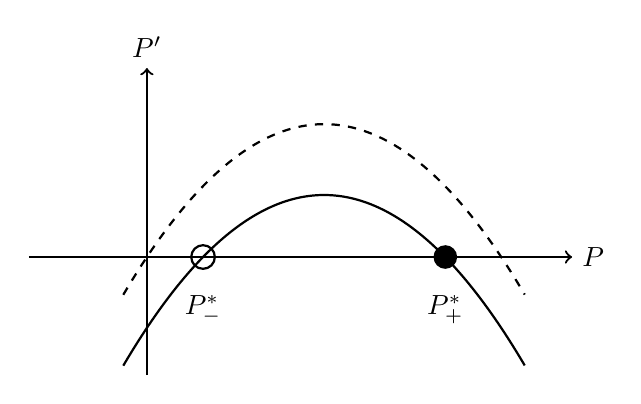
\begin{tikzpicture}[scale=3]
\begin{scope}
    % Axes
        % arrows: x<0 left
    % \draw[->,thick] (-0.3,0) -- (-0.4,0);
    % arrows: 0<x<1 right
    % \draw[->,thick] (0.4,0) -- (.6,0);
    % arrows: x>1 left
    % \draw[->,thick] (1.4,0) -- (1.3,0);
    % Axes
    \draw[->,thick] (-0.5,0) -- (1.8,0) node[right] {$P$};
    % \draw[very thick,blue] (-0.5,0) -- (0,0);
    % \draw[very thick,blue] (1,0) -- (1.5,0);
    % \draw[very thick,red] (0,0) -- (1,0);
    \draw[->,thick] (0,-.5) -- (0,.8) node[above] {$P'$};
    \draw[thick,dashed,domain=-0.1:1.6,samples=100] plot (\x,{ \x*(1.5-\x)});
    \draw[thick,domain=-0.1:1.6,samples=100] plot (\x,{ \x*(1.5-\x)-0.3});
    % \node[right] at (0.5,0.5) {$f(P)=0.4\,P(1-\frac{P}{10000})$};
    %     \node[below] at (0,-0.12) {$0$};
    % \node[below] at (1,-0.12) {$10000$};
    %     \fill (1,0) circle (0.05);
    %     \draw[thick] (0,0) circle (0.05);\textbf{}
        \draw[thick] (0.2377,0) circle (0.05);
        \node[below] at (0.2377,-0.12) {$P^*_-$};
        \fill (1.2633,0) circle (0.05);
        \node[below] at (1.2633,-0.12) {$P^*_+$};
\end{scope}
\end{tikzpicture}\caption{This is the $P'$ vs. $P$ graph for the logistic model with harvesting. The left equilibrium $P^*_-$ is unstable and the right $P^*_+$ is stable}
\end{figure}


%-------------------------------------------------------------
\section{Fixed Population Models}
So far, our population models have described how the total size of a
population changes. We can also model how individuals \textit{move between
groups} within a population.

% In many applications, we model a system where individuals move between categories, but the total population stays fixed. We'll call these  \textit{fixed population models}. Examples include:
% \begin{itemize}
%     \item people switching health states (sick, healthy),
%     \item people changing religions,
%     \item chemicals switching molecular states,
%     \item information spreading in a network,
%     \item customers switching subscription tiers.
% \end{itemize}
% The key idea is that individuals are not created or destroyed; they only change category.

%-------------------------------------------------------------
\subsection{Two Groups}


Suppose a population of $N$ individuals is divided into two groups:
\[
A(t)=\text{number of individuals in group $A$},
\qquad
B(t)=\text{number of individuals in group $B$}.
\]
Although $A(t)$ and $B(t)$ may change over time, we assume that the total population is fixed:
\[
A(t)+B(t)=N.
\]
Individuals may move between the two groups. For example, an individual from group $B$ can leave and enter group $A$. Thus, as one group gains individuals, the other group loses them.

%-------------------------------------------------------------
\subsection{Goal}

Our goal is to develop a model that describes how the two groups change over
time. In other words, we want to develop differential equations for
\[
A'(t)
\qquad\text{and}\qquad
B'(t).
\]
The equations will depend on how individuals move between groups $A$ and $B$.

% ----------------------------------------------------

\begin{example}[4]{
A company has $1000$ customers divided between two subscription plans:
Basic and Premium. Each month, $10\%$ of Basic customers upgrade to Premium,
while $5\%$ of Premium customers downgrade to Basic. Develop a fixed population model for
the number of Basic and Premium customers.
}

Let $B(t)$ and $P(t)$ be the number of Basic and Premium customers, respectively.
Since the total number of customers is fixed, we let $B(t)+P(t)=1000$. 

Each month, $10\%$ of the Basic customers upgrade to Premium. Therefore,
$B$ decreases at a rate of $0.10B$, while $P$ increases at the same rate:
\[
B'=-0.10B+\ldots,
\qquad
P'=0.10B+\ldots.
\]
Similarly, $5\%$ of the Premium customers downgrade to Basic. Therefore,
$P$ decreases at a rate of $0.05P$, while $B$ increases at the same rate:
\[
B'=-0.10B+0.05P,
\qquad
P'=0.10B-0.05P.
\]
Therefore, the model is
\[
\boxed{
\begin{dcases}
B'=-0.10B+0.05P,\\
P'=\phantom{-}0.10B-0.05P.
\end{dcases}
}
\]
\end{example}

%-------------------------------------------------------------
\subsection{Fixed Population Constraint}

In a fixed population model,
\[
A(t)+B(t)=N.
\]
Therefore, the two populations are not independent. If we know one
population, we automatically know the other:
\[
B(t)=N-A(t).
\]
There is also a corresponding relationship between the rates of change.
Differentiating $A+B=N$ gives
\[
A'(t)+B'(t)=0 \implies A' =-B'.
\]
For instance, in Example 3, we had $B'=-0.10B+0.05P = -P'$.  
This means that a model with two subpopulations can be reduced to a single differential equation. In the previous example, the number of Premium customers is 
\[
P(t)=1000-B(t).
\]
Substituting $P$ into the equation for $B'$ yields 
$$
B'=-0.10B+0.05P =-0.10B+0.05(1000-B)=500-0.15B.
$$
This new DE has the form 
$$
B'=f(B)
$$
which is an autonomous equation.

%-------------------------------------------------------------
\subsection{Interaction Terms}

Sometimes the rate at which individuals change groups depends on
\textit{interactions} between the two groups. Suppose an individual from group $A$ must interact with an individual from group $B$ before either can change groups. The frequency of these interactions is proportional to the product
\[
AB.
\]
We, therefore, model the interaction rate by
\[
kAB,
\]
where $k>0$ is an \textbf{interaction rate}. The larger either group becomes, the more opportunities there are for
individuals from the two groups to interact.

% \subsection{Example}
% The year is 2019. There are 100 students living in a dorm, and they're all friendly with each other. We can break them up into two categories 
% \begin{align*}
% &A(t)=\text{people who have seen the show Game of Thrones},\\
% &B(t)=\text{people who have not seen Game of Thrones},
% \end{align*}
% with $A(t)+B(t)=100$.
% GOT fans are relentless. Whenever a student from group $A$ interacts with a student from group $B$, the student in group $A$ pressures the other into watching the show. We can model the population as 
% \[
% \begin{dcases}
% A' = k\,AB\\
% B' = -k\,AB,
% \end{dcases}
% \]
% where $k>0$ is an interaction rate. The multiplication $AB$ represents the meeting of two people in each group. The parameter $k$ controls the frequency of the encounter. $A'$ is proportional to $AB$ because when a person watches the show, they are moved to converted to group $A$. For the same reason, $B'$ is proportional to $-AB$.

% Let's say the interaction term is $k=2$ per day per person. Let's assume there are 2 people in group $A$. What happens to the to the population of groups $A$ and $B$?

% \subsection{Solution}
% If only 2 students have seen the show, the initial condition is $A(0)=2$ and $B(0)=98$. Since the total population is fixed,
% \[
% B(t)=100-A(t).
% \]
% Substituting into the equation for $B$ gives a single differential equation:
% \[
% A' = kAB = kA(N-A) = 2\,A(100-A).
% \]
% This model has an equilibrium at $A^*=0$ and $A^*=100$. Plotting $A'$ versus $A$ shows gives us the phase line. The phase line shows that $A^*=100$ is stable. Even if you start with an initial population as low as $A(0)=2$, the population of $A$ eventually reaches 100. This model is actually exactly the same as the logistic growth model. The big difference is that the population cannot exceed $A=100$ which would be the carrying capacity in the other model. 
% \begin{figure}[H]
%     \centering
% \begin{tikzpicture}[scale=3]
% \begin{scope}
%     % Axes
%         % arrows: x<0 left
%     \draw[->,thick] (-0.3,0) -- (-0.4,0);
%     % arrows: 0<x<1 right
%     \draw[->,thick] (0.4,0) -- (.6,0);
%     % arrows: x>1 left
%     \draw[->,thick] (1.4,0) -- (1.3,0);
%     % Axes
%     \draw[->,thick] (-0.5,0) -- (1.8,0) node[right] {$A$};
%     \draw[very thick,blue] (-0.5,0) -- (0,0);
%     \draw[very thick,blue] (1,0) -- (1.5,0);
%     \draw[very thick,red] (0,0) -- (1,0);
%     \draw[->,thick] (0,-.1) -- (0,0.7) node[above] {$A'$};
%     % Curves x(t) = C e^{-t}
%     \draw[thick,domain=-0.2:1.2,samples=100] plot (\x,{ \x*(1-\x)});
%     \node[right] at (0.5,0.5) {$f(A)=2\,A(100-A)$};
%         \node[below] at (0,-0.12) {$0$};
%     \node[below] at (1,-0.12) {$100$};
%         \fill (1,0) circle (0.05);
%         \draw[thick] (0,0) circle (0.05);
% \end{scope}
% \end{tikzpicture}\caption{This is the $A'$ vs. $PA$ graph and phase line combined in one. The equilibrium $A^*=100$ is stable.}
% \end{figure}
% Here are some comments about this type of problem:
% \begin{itemize}
%     \item We assumed $A$ and $B$ are integers. Usually, we scale everything by $N$ to make $A$ and $B$ a percentage. 
%     \item When there are only two groups in a fixed-population model, their DE's are mirrored. They have the same terms with opposite signs. 
%     \item You don't have to solve for $B(t)$. Solving for $A(t)$ is enough because you get the other for free $B(t) = N-A(t)$. 
%     \item What if a person watches GOT but doesn't like the show? We may want to add a third group $C(t)$ to account for that.
% \end{itemize}

\subsection*{SIR Model}
Fixed-population models are frequently used in epidemiology. Scientists use \textbf{SIR model} to study a population of people with an infectious disease. A common example is a flu. Here are the groups:
\begin{itemize}
    \item $S(t)$ = number of people that are susceptible 
    \item $I(t)$ = number of people that are infected
    \item $R(t)$ = number of people that have recovered and developed immunity
\end{itemize}
The sum of each subpopulation must add up to a total of $N$ at all times. A sick person may randomly encounter a healthy person. When this happens, the sick person transmits the disease to the healthy person. A sick person can eventually recover with their immune system. When a person overcomes the disease, they gain immunity from it so they do not catch the disease again. A simplified model would be 
$$
\begin{dcases}
    S' &= -kIS,\\
    I' &= kIS - rI,\\
    R' &= rI,
\end{dcases}
$$
where $k$ and $r$ are positive constants. The product $kIS$ represents the encounter between a sick person and a healthy person. The parameter $r$ represents how quickly a person overcomes the flu. There are many variants of this model. For example, there could be a deceased group or a vaccinated group. We may have a group of carriers that don't show any symptoms.
\end{document}
